
\section{Road Generation}\label{sec:road-generation}

\renewcommand{\kapitelautor}{Autor: Felix Zwickelstorfer}

Die Generierung von Straßen ist ein sehr wichtiger Punkt in Forty-Five, da es bei einem neuen Durchlauf für Abwechslung für den Spieler sorgt.
Es gibt bei der Erstellung von Roads bestimmte Parameter, damit trotzdem noch bestimmte Randbedingungen erfüllen wie beispielsweise, dass immer die gleichen Texturen als Dekorationen verwendet werden.
Im Folgenden wird nun die Entstehung einer Straße und die dabei gesetzten Parameter näher gebracht.

\subsection{Node Generation}\label{subsec:node-generation}
Um eine Straße zu generieren, braucht man als erstes Nodes, also Punkte in einem Koordinatensystem.
Diese werden wiederum anhand von sogenannten \inlineCode{MapNodeLine} erstellt und anschließend miteinander verbunden.

\subsubsection{Line Generation}\label{subsubsec:line-generation}
Eine Linie nimmt mehrere Parameter: die Anzahl der nodes, die Abstände dazwischen, und die maximale Breite, welche eine Linie zur Verfügung hat.
Linien werden immer in Richtung rechts gebaut, und erst am Ende wird die gesamte Road rotiert.
Die erste Linie, die generiert wird, funktioniert etwas anders als die anderen, da diese weniger Einschränkungen hat.
Dies geschieht folgendermaßen:

\begin{enumerate}
    \item Die Hauptlinie wird als erstes erstellt und beginnt mit dem Punkt (0|0).
    \item Es werden n weitere Punkte generiert, wobei folgende Kriterien gelten, die alle als Einschränkungen der Map angegeben werden:
    \begin{itemize}
        \item Er hat einen Mindest- und Maximalabstand in sowohl x als auch y Richtung vom vorherigen Punkt.
        \item Er hat einen maximalen Winkel vom vorherigen Punkt.
        \item Er kann hat einen maximalen Breitenabstand zu dem ersten Punkt auf der Linie.
    \end{itemize}
    \item Anschließend wird eine zufällige Richtung ausgewählt, in der die nächste Linie generiert wird, entweder darüber oder darunter.
    Diese ist immer um genau einen Punkt kürzer als die davor.
    Das stellt sicher, dass keine Linie länger sein kann als die Hauptlinie, und dass es im Normalfall auch nicht zu stark am Ende abschneidet.
    \item Der neue Startpunkt ist die Hälfe eines normalen Punktes in x-Richtung und dann um die maximal erlaubte Breite in y-Richtung nach oben oder unten, je nachdem was davor entschieden wurde.
    \item Anschließend werden wieder gleich die Nodes berechnet wie bei der Hauptlinie, nur dass ein zusätzlicher Punkt dazukommt:
    Der Abstand zu der davorliegenden Linie darf in einem Bereich um den zu planierenden Punkt nicht zu weit entfernt sein.
    Dies vermeidet, dass die Abstände zwischen zwei Linien nicht zu groß sind und dadurch auseinandergehen.
    Dies wird an der darauffolgenden Grafik gezeigt.
    \item Dann werden Punkt drei bis fünf so oft generiert, wie \inlineCode{maxLines} angibt.
\end{enumerate}

% TODO BILD BESCHREIBEN

\begin{figure}[H]
    \centering
    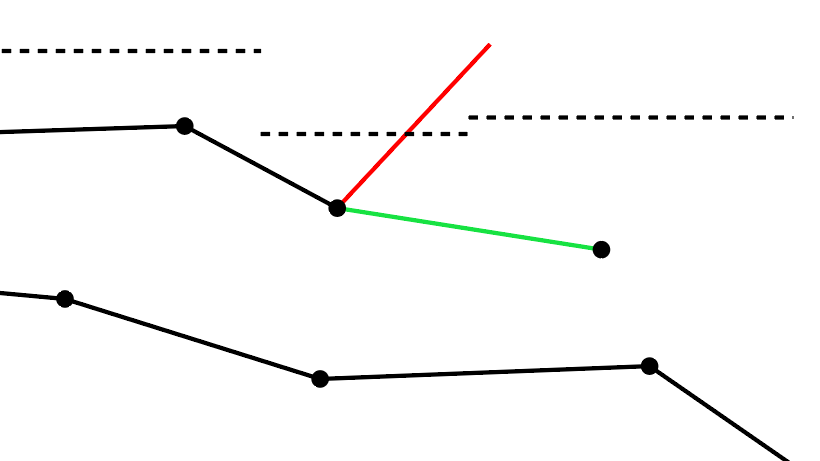
\includegraphics[width=0.7\textwidth]{node_generation_example.png}
    \caption{Beispiel: Punktegenerierung mit Fehlerhafter Platzierung }
\end{figure}


\subsubsection{Node Verbindungen}\label{subsubsec:node-verbindungen}
Nachdem nun eine Sammlung an Nodes vorhanden ist, werden diese miteinander Verbunden.
Dabei bekommt jedes Node einen Freien Platz für jede Richtung, damit nicht zu viele Nodes in die gleiche Richtung miteinander verbunden werden.
Außerdem wird dadurch die maximale Anzahl an Verbindungen pro Node auf vier limitiert, da man auch nur vier